\begin{homework}
    \begin{questions}
        \Question[10] Calculate:
        \begin{parts}
                \part \(226+601+478=\fillin[]\)
                \part \(72 \div 3=\fillin[]\)
                \part \(163-136=\fillin[]\)
                \part \(20 \div(9-4)+6=\fillin[]\)
                \part \(8 \times 321+6=\fillin[]\)
                \part \(68-42+12 \times 2=\fillin[]\)
                \part \(382-792 \div 3=\fillin[]\)
                \part \(268 \times(3+7)=\fillin[]\)
                \part \((96 \div 3)+(258 \div 3)=\fillin[]\)
        \end{parts}
        \Question[2] The contents of a tin of chocolates weigh 6500 grams. The chocolates are divided into packets of 250 grams. How many packets are there?
            \begin{solutionordottedlines}[2in]
            \end{solutionordottedlines}
        \Question[2] There are 4000 apples to be divided into boxes so that each box holds 75 apples. How many boxes are required?
            \begin{solutionordottedlines}[2in]
            \end{solutionordottedlines}
        \Question[2] A club started the year with 125 members. During the year, 23 people left and 68 people joined. How many people belonged to the club at the end of the year?
            \begin{solutionordottedlines}[2in]
            \end{solutionordottedlines}
        \Question[2] If a bus can carry 45 passengers, how many buses are needed to transport 670 school students to a hockey game?
            \begin{solutionordottedlines}[2in]
            \end{solutionordottedlines}
        \Question[2] A supermarket takes delivery of 54 cartons of soft drink cans. Each carton contains 48 cans. How many cans are delivered?
            \begin{solutionordottedlines}[2in]
            \end{solutionordottedlines}
        \Question[2] On a school excursion, 17 buses each carry 42 students. How many students are transported?
            \begin{solutionordottedlines}[2in]
            \end{solutionordottedlines}
        \Question[2] A school day is 6 hours long. How many minutes are there in a school day?
            \begin{solutionordottedlines}[2in]
            \end{solutionordottedlines}
        \Question[2] Find the sum of eighty-six and fifty-four and then subtract sixty-eight.
            \begin{solutionordottedlines}[2in]
            \end{solutionordottedlines}
        \Question[2] The manager of the school canteen orders 1000 hot dogs for the week. On Monday 384 are sold and on Tuesday 239 are sold. How many hot dogs does the school have left for the rest of the week?
            \begin{solutionordottedlines}[2in]
            \end{solutionordottedlines}
        \Question[2] Use five \(6 \mathrm{~s}\) and a selection of the symbols \[ (,),+,-, \times \text { and } \div \] to write a statement with 66 as the result.
            \begin{solutionordottedlines}[2in]
            \end{solutionordottedlines}
    \end{questions}
\end{homework}
\begin{challenge}
    \begin{questions}
        \Question[3] Place the numbers 1 to 9 in the circles to make each of the equations true.
        \begin{center}
            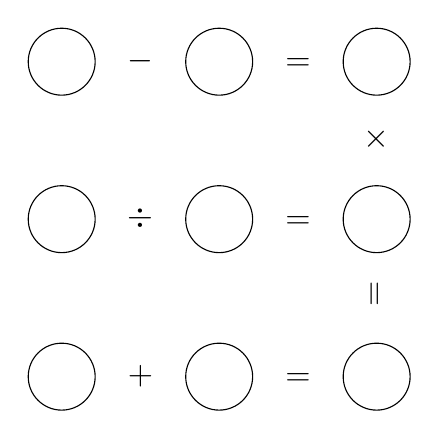
\begin{tikzpicture}
              % Define styles for circles and symbols
              \tikzset{
                circle node/.style={circle, draw, minimum size=0.85cm},
                symbol node/.style={font=\large, text height=1.5ex}
              }

              % First row
              \node[circle node] (c11) at (0,2) {};
              \node[symbol node] (s11) at (1,2) {$-$};
              \node[circle node] (c12) at (2,2) {};
              \node[symbol node] (eq1) at (3,2) {$=$};
              \node[circle node] (c13) at (4,2) {};
              \node[symbol node] (x1) at (4,1) {$\times$};

              % Second row
              \node[circle node] (c21) at (0,0) {};
              \node[symbol node] (s21) at (1,0) {$\div$};
              \node[circle node] (c22) at (2,0) {};
              \node[symbol node] (eq2) at (3,0) {$=$};
              \node[circle node] (c23) at (4,0) {};
              \node[symbol node] (div1) at (4,-1) {\rotatebox{90}{$=$}};

              % Third row
              \node[circle node] (c31) at (0,-2) {};
              \node[symbol node] (s31) at (1,-2) {$+$};
              \node[circle node] (c32) at (2,-2) {};
              \node[symbol node] (eq3) at (3,-2) {$=$};
              \node[circle node] (c33) at (4,-2) {};
            \end{tikzpicture}
        \end{center}
        \Question[3] Find the missing digits in the following multiplication.
        \par\centering
            \begin{tabular}{ccccccc}
                        & & & &$\star$&$\star$&$\star$\\
                $\times$& & & &$\star$&2&$\star$\\
                \hline\\
                        & & & &$\star$&$\star$&$\star$\\
                        & &$\star$&$\star$&$\star$&$\star$&0\\
                        & &$\star$&8&$\star$&0&0\\
                \hline\\
                        &$\star$&$\star$&9&$\star$&2&$\star$\\
                \hline
            \end{tabular}
            \begin{solutionorbox}[2in]
            \end{solutionorbox}
        \Question[3] Use all of the numbers \(1,2,3,4,5,6\) and 7 once and the symbols,\(+,-,\times\) and \(\div\) to make a number sentence that results in 100 .
            \begin{solutionorbox}[2in]
            \end{solutionorbox}
        \Question[4] A fast food store sells nuggets in boxes of 5 and 8 . You can buy 31 nuggets at a time since \(3 \times 5+2 \times 8=31\). What is the largest whole number of nuggets that cannot be purchased?
            \begin{solutionorbox}[2in]
            \end{solutionorbox}
        \Question[4] It is possible to choose four numbers such that any value between 1 and 40 can be made by taking one or more of these numbers and adding or subtracting them from each other. Find the four numbers, and show how the values from 1 to 40 can be made.
            \begin{solutionorbox}[2in]
            \end{solutionorbox}
    \end{questions}
\end{challenge}
